\chapter{提案手法}
\label{chap:proposed_method}

本章では，オノマトペの音象徴をロボットの歩行動作へ反映する提案手法について述べる．
本研究で扱う課題は，抽象的な言語表現と物理的なロボット制御という，性質の大きく異なる要素を統合する点にある．

これらを単一の枠組みで直接結びつけることは容易ではない．
特に，学習データに含まれない未知のオノマトペに対しても適切な動作を生成するためには，
言語と動作を共通の概念空間へ写像し，未知の表現に対しても汎化可能な特徴を獲得する必要がある．
そこで本手法では，まず対照学習によって言語と動作の共有潜在空間を構築して未知語への対応力を高め，
その後に獲得した表現に基づいて強化学習を行う二段階構成を採用する．構成は次の順に整理する．

\begin{enumerate}
  \item HOYO に対する前処理
  \item 対照学習による言語--動作整合（Phase 1）
  \item 強化学習によるスタイル制御（Phase 2）
\end{enumerate}
以下では，まず全体像（\ref{sec:system_overview}）と問題定式化（\ref{sec:formulation}）を示し，
HOYO 前処理（\ref{sec:preprocess}），Phase 1（\ref{sec:offline_phase}），Phase 2（\ref{sec:online_phase}）の順に詳細を述べる．

\section{手法の全体像}
\label{sec:system_overview}

提案手法はオフライン表現学習とオンライン強化学習の 2 段階で構成される（図\ref{fig:overview}）．

\begin{figure}[H]
  \centering
  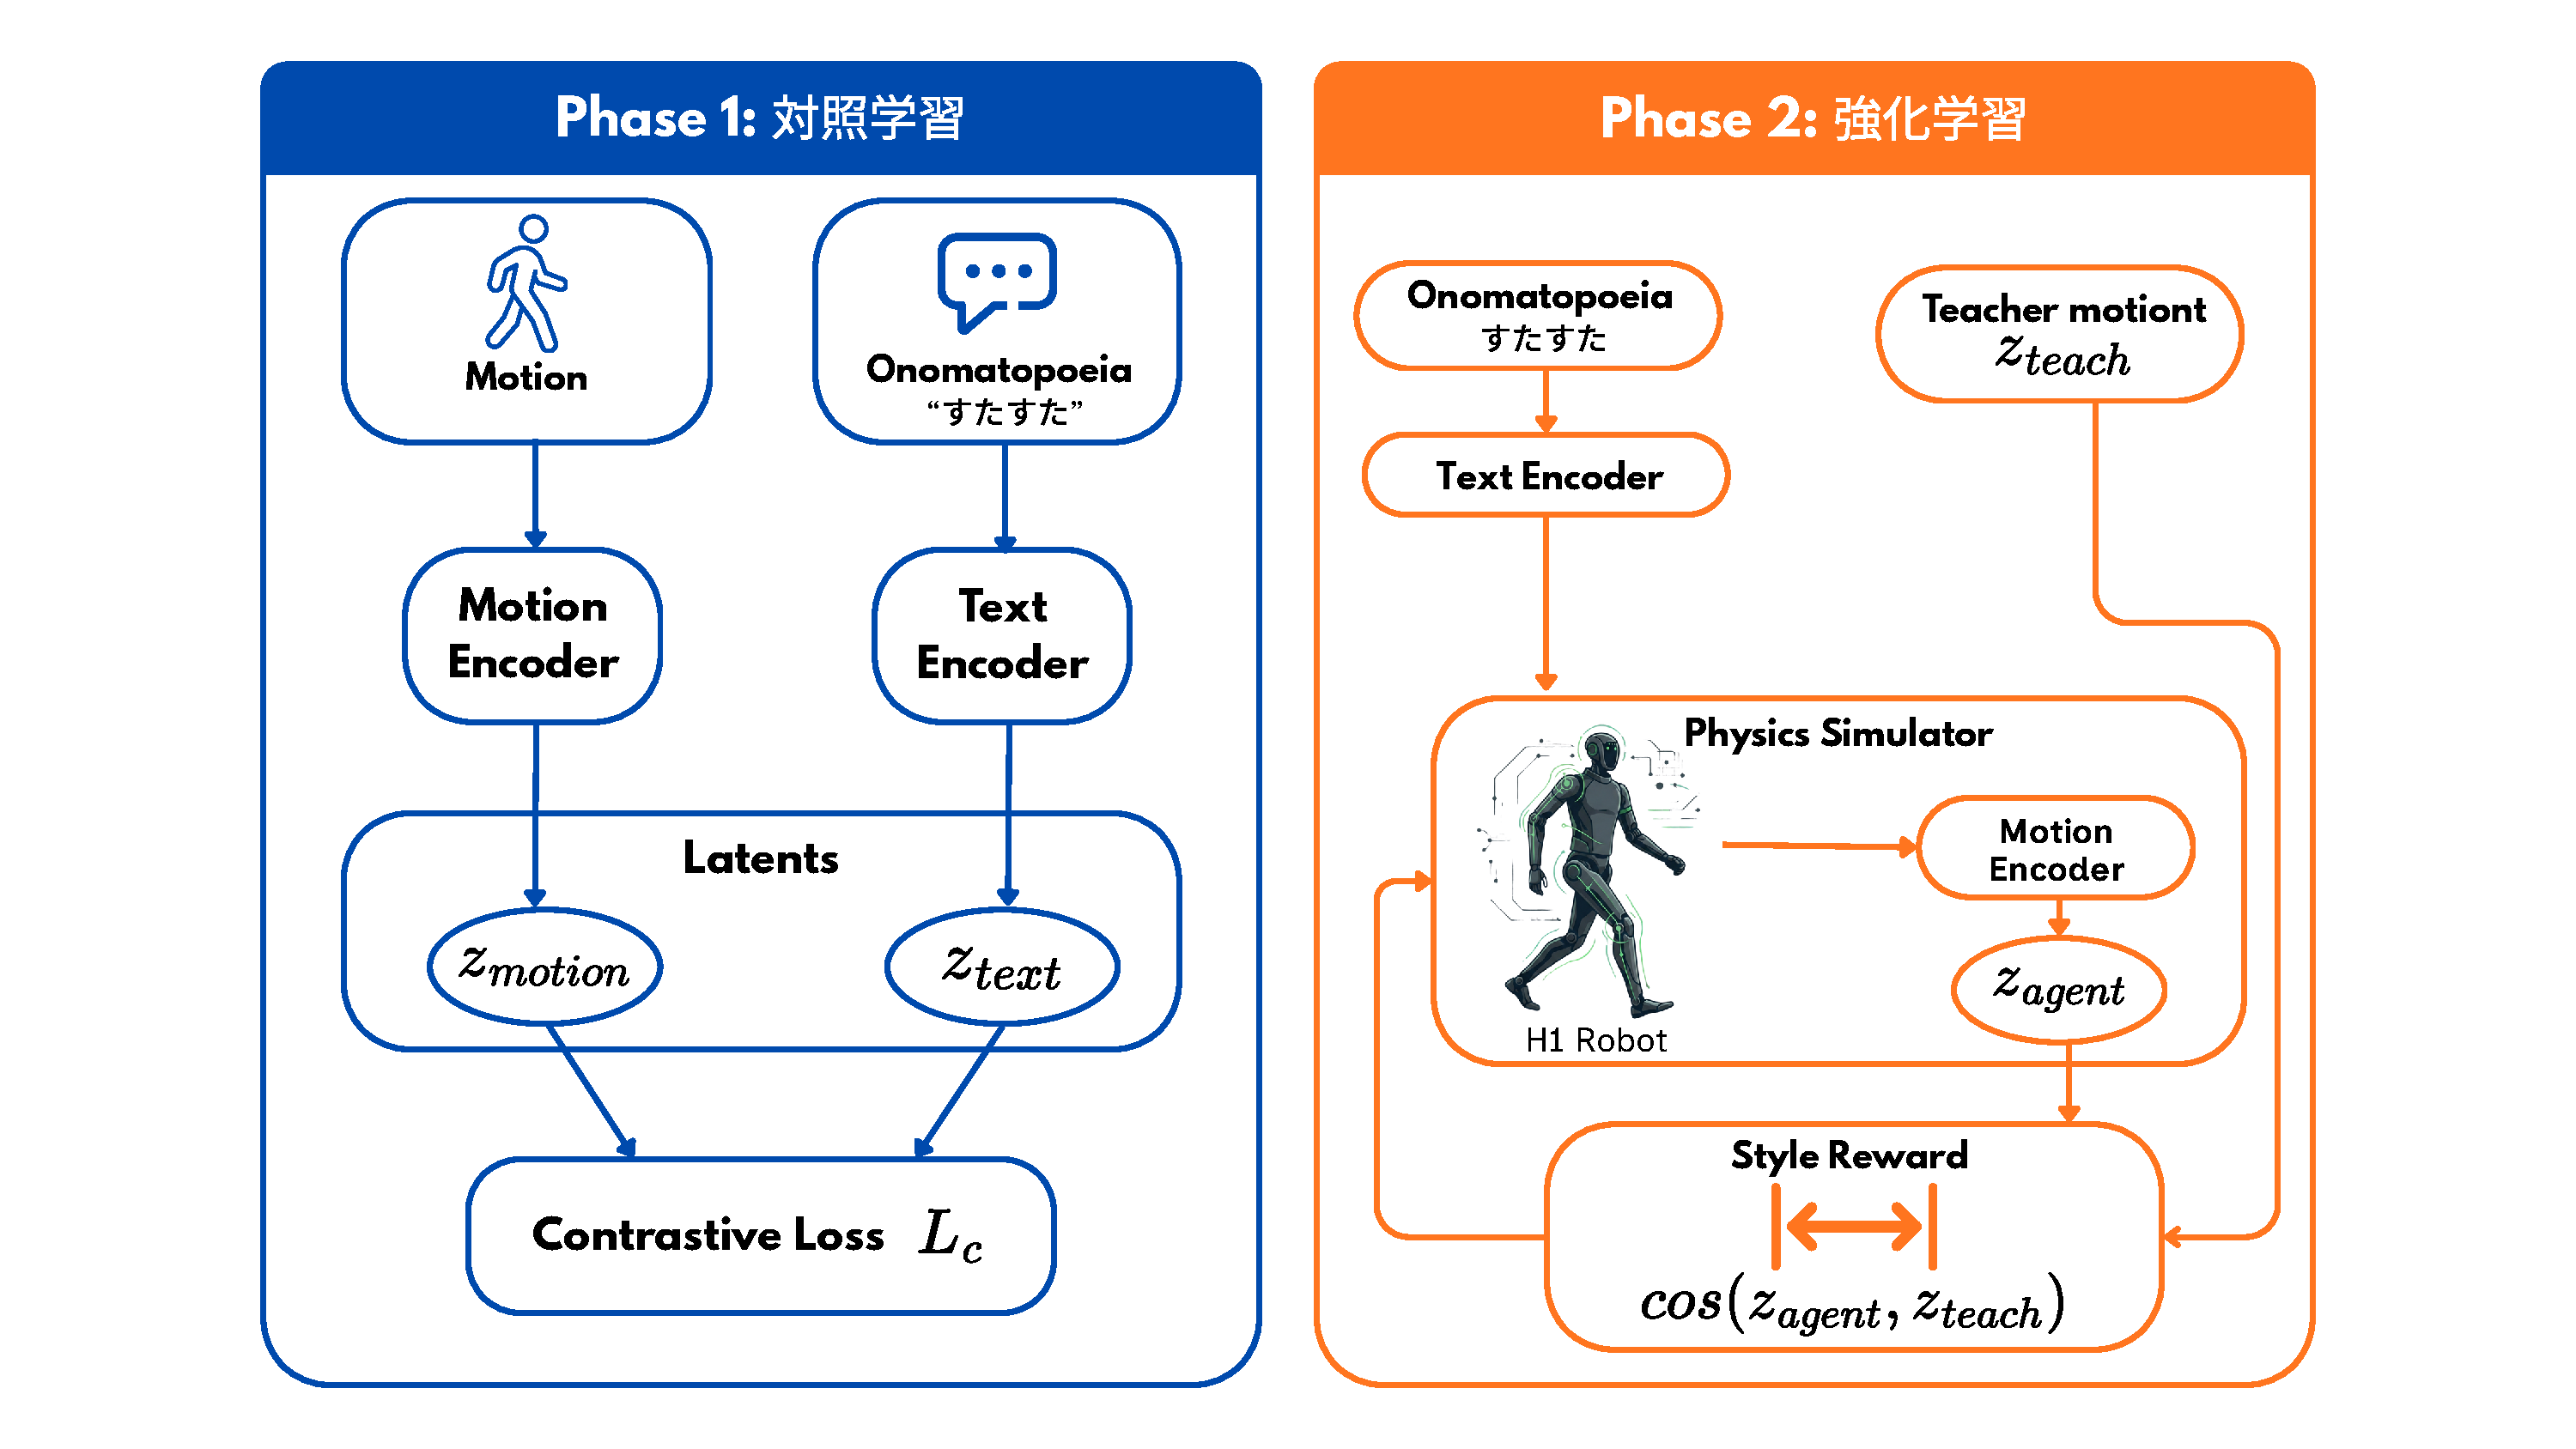
\includegraphics[width=\textwidth]{figs/3/Model_Abstract.pdf}
  \caption{提案手法の全体構成（Phase 1: 対照学習／Phase 2: 強化学習）}
  \label{fig:overview}
\end{figure}

\begin{enumerate}
  \item \textbf{Phase 1（対照学習）}：\leavevmode\\
        HOYO \cite{hoyo} の 2D 歩容系列とオノマトペを用い，MotionCLIP \cite{MotionCLIP} を基盤とした共有潜在空間を構築する．
        変分オートエンコーダ（VAE）による再構成と，教師あり対照学習による意味整合を同時に学習する．

  \item \textbf{Phase 2（強化学習）}：\leavevmode\\
        物理シミュレータ（Isaac Lab）上のヒューマノイドロボット（H1）に対し，PPO により歩行方策を学習する．
        ロボット動作を HOYO 形式の 2D 系列へリターゲットし，Phase 1 のエンコーダで評価した類似度をスタイル報酬として与える．
\end{enumerate}

\section{問題定式化}
\label{sec:formulation}

各サンプルは 2D 歩容系列 $X\in\mathbb{R}^{T\times J\times 2}$ と
オノマトペ $w$ の組 $(X,w)$ で与えられる．
運動系列をエンコーダで埋め込み
\begin{align}
  z_{\mathrm{mot}}=\mathrm{normalize}\!\left(f_{\mathrm{enc}}(\tilde{X})\right)
\end{align}
を得る．ここで $\tilde{X}$ は前処理後の系列である．
テキスト側はテンプレート文 $\mathrm{text}(w)$ を用いて埋め込み
\begin{align}
  u_{\mathrm{sem}} = e_{\mathrm{text}}(\mathrm{text}(w)),\quad
  z_{\mathrm{sem}}=\mathrm{normalize}(W u_{\mathrm{sem}})
\end{align}
を得る．
Phase 1 では再構成損失 $\mathcal{L}_{\mathrm{VAE}}$ と
対照損失 $\mathcal{L}_{\mathrm{con}}$ を併用し，
\begin{align}
  \mathcal{L}_{\mathrm{total}}
  = \lambda_{\mathrm{vae}}\,\mathcal{L}_{\mathrm{VAE}}
  + \lambda_{\mathrm{con}}\,\mathcal{L}_{\mathrm{con}}
\end{align}
を最小化する．$\mathcal{L}_{\mathrm{con}}$ は SupCon を用いる．

Phase 2 では方策 $\pi_\theta$ がスタイル報酬を最大化するよう学習される．
目標は
\begin{align}
  J(\pi_\theta)=\mathbb{E}_{\pi_\theta}\!\left[\sum_{t=0}^{\infty}\gamma^t r_t\right]
\end{align}
であり，報酬 $r_t$ の具体形は \ref{subsec:rl_reward} 節で定義する．

\subsection{歩容スタイルの定義と潜在空間で扱う意義}
\label{subsec:gait_style_definition}

本研究でいう「歩容スタイル」とは，オノマトペが表す歩行印象
（例：速さ感，重さ感，揺れ方）を反映した運動特徴の総体を指す．
HOYO \cite{hoyo} では，同じオノマトペに対しても複数の被験者サンプルが含まれるため，
ラベル内には体格や癖に由来する個人差が含まれる．
したがって本研究の目的は，個人固有の運動そのものを再現することではなく，
同一オノマトペに共通する歩容特徴を抽出して「語彙レベルのスタイル」を学習することである．
以降，「スタイル」は特記がない限り歩容スタイルを意味する．

この目的に対して，共有潜在空間での対照学習には次の意義がある．
MotionCLIP \cite{MotionCLIP} に基づく潜在表現へモーションと言語を写像し，
同一オノマトペを正例として引き寄せ，異なるオノマトペを負例として分離することで，
個人差に起因するばらつきを抑えつつ語彙に共通する歩容特徴を強調できる \cite{supcon}．
これにより，未知オノマトペに対しても，意味的に近い既知語の近傍へ配置することで
歩容スタイルの一般化を狙う．

\section{前処理：HOYO データセット}
\label{sec:preprocess}

\subsection{データセット概要}
\label{subsec:preprocess_flow}

HOYO \cite{hoyo} は，歩行動画に対してオノマトペのラベルが付与された 2D 歩容データセットである．
各動画から Convolutional Pose Machines（CPM）により検出した 14 箇所の部位座標列が，
歩容スケルトンとしてデータセットに含まれている．
図\ref{fig:hoyo_dataset}に HOYO データセットの元動画と歩容スケルトンを示す．

\begin{figure}[tbp]
  \centering
  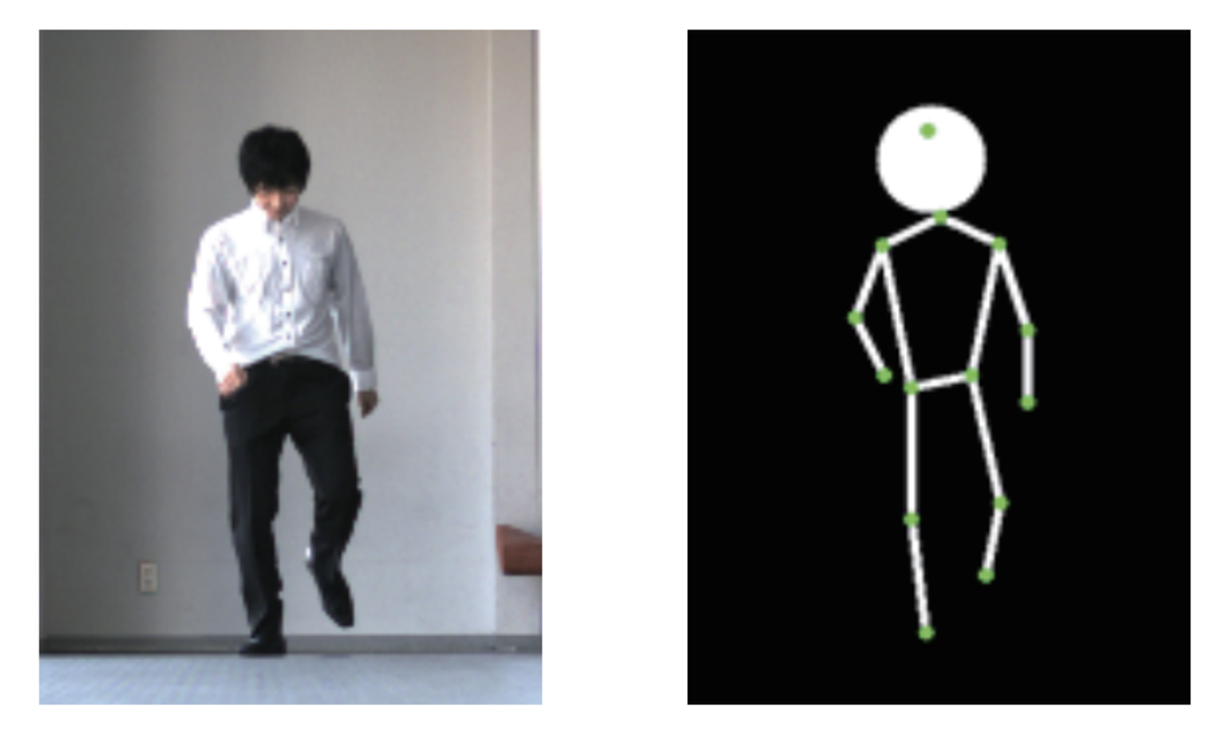
\includegraphics[width=0.9\linewidth]{figs/3/hoyo_dataset.pdf}
  \caption{HOYO データセットの元動画と歩容スケルトン（\cite{hoyo}より引用）}
  \label{fig:hoyo_dataset}
\end{figure}


本研究では HOYO の定義に従い，関節数 $J=14$ の 2D スケルトン系列を用いる．

各サンプルはフレーム長 $T$ の系列 $X \in \mathbb{R}^{T \times J \times 2}$ として表される．
教師データとして，HOYO に含まれる 11 種類のオノマトペ（通常，すたすた，せかせか，てくてく，どっしどっし，とぼとぼ，のしのし，のろのろ，ぶらぶら，よたよた，よろよろ）を用いる．

\subsection{前処理の手順}
\label{subsec:preprocess_steps}

ロボットの学習に適した形式に変換するため，以下の前処理を適用する．
前処理フローの全体像を図\ref{fig:hoyo_preprocessing}に示す．

\begin{figure}[htbp]
  \centering
  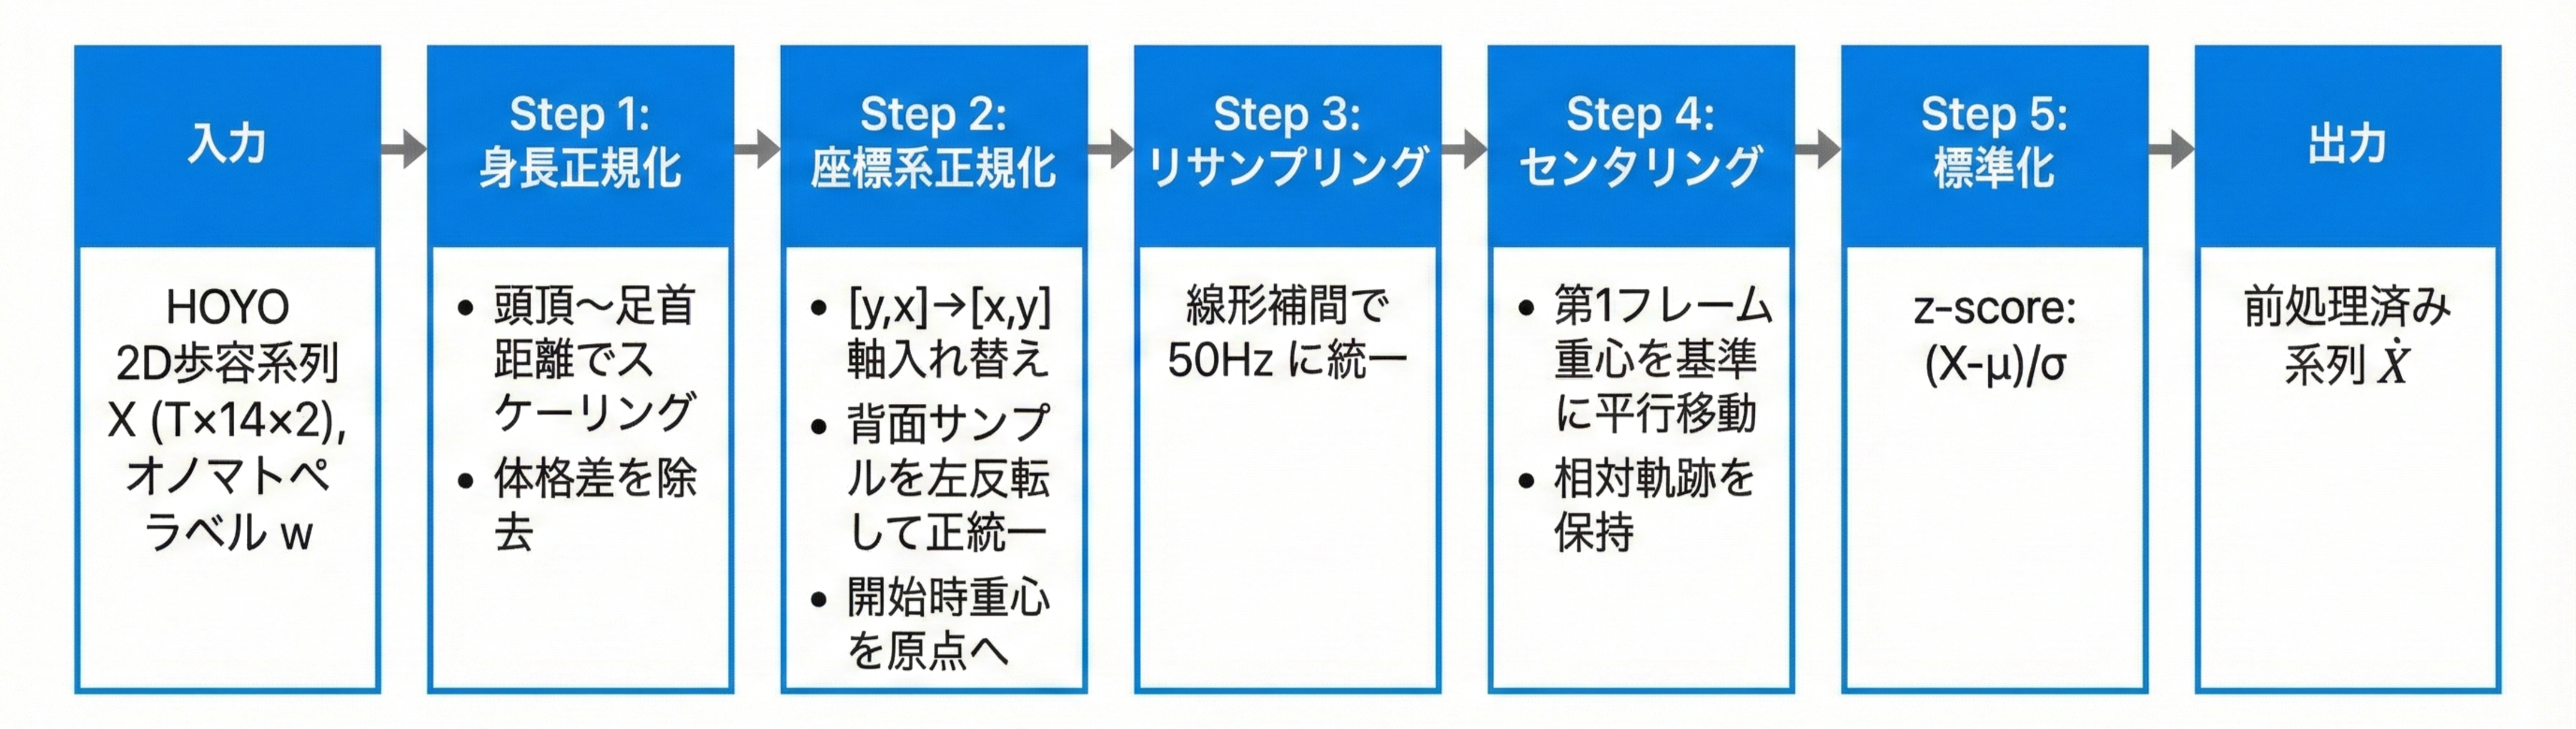
\includegraphics[width=\textwidth]{figs/3/hoyo_preprocessing.pdf}
  \caption{HOYO 2D 歩容系列に対する前処理フロー}
  \label{fig:hoyo_preprocessing}
\end{figure}

\begin{enumerate}
  \item \textbf{身長正規化}\par
        被験者の体格差による影響を排除するため，身長に基づく正規化を行う．
        頭頂と足首の平均距離から身長スケールを推定し，関節座標全体を除算することで，
        身体の大きさに依存しない正規化された骨格系列を得る．
  \item \textbf{座標系の正規化}\par
        HOYO の画像座標系から，ロボット制御で一般的な座標系へ変換を行う．
        具体的には，座標軸を $[y, x] \to [x, y]$ へ入れ替えるとともに，
        背面から撮影されたサンプルについては左右反転処理を行い，すべてのデータを正面ビューに統一する．
  \item \textbf{リサンプリング}\par
        動画データのフレームレート（FPS）と強化学習のシミュレータ上の
        ロボットの制御周期を一致させるため，線形補間を用いて系列を 50 Hz にリサンプリングする．
  \item \textbf{センタリング}\par
        ロボットのローカルな姿勢制御とグローバルな移動を分離して学習させるため，
        センタリングを採用する．
        これは，系列の第 1 フレームの重心位置を初期位置として差し引き，重心を原点に揃えることを目的とする．
        その結果，絶対座標の影響を除きつつ，歩行に伴う重心移動の相対軌跡は保持される．
  \item \textbf{標準化}\par
        ニューラルネットワークの入力分布を安定させるため，全学習データの平均 $\mu$ および
        標準偏差 $\sigma$ を算出・保存し，$z$-score 正規化（$\tilde{X}=(X-\mu)/\sigma$）を適用する．
\end{enumerate}




\section{対照学習による言語--動作整合（Phase 1）}
\label{sec:offline_phase}

本節では，前節の前処理済み系列を入力とし，\textbf{モデル構成}と\textbf{学習手順}を整理する．
Phase 1 における入力から潜在空間学習までの流れを図\ref{fig:phase1_contrastive_learning}に示す．

\begin{figure}[htbp]
  \centering
  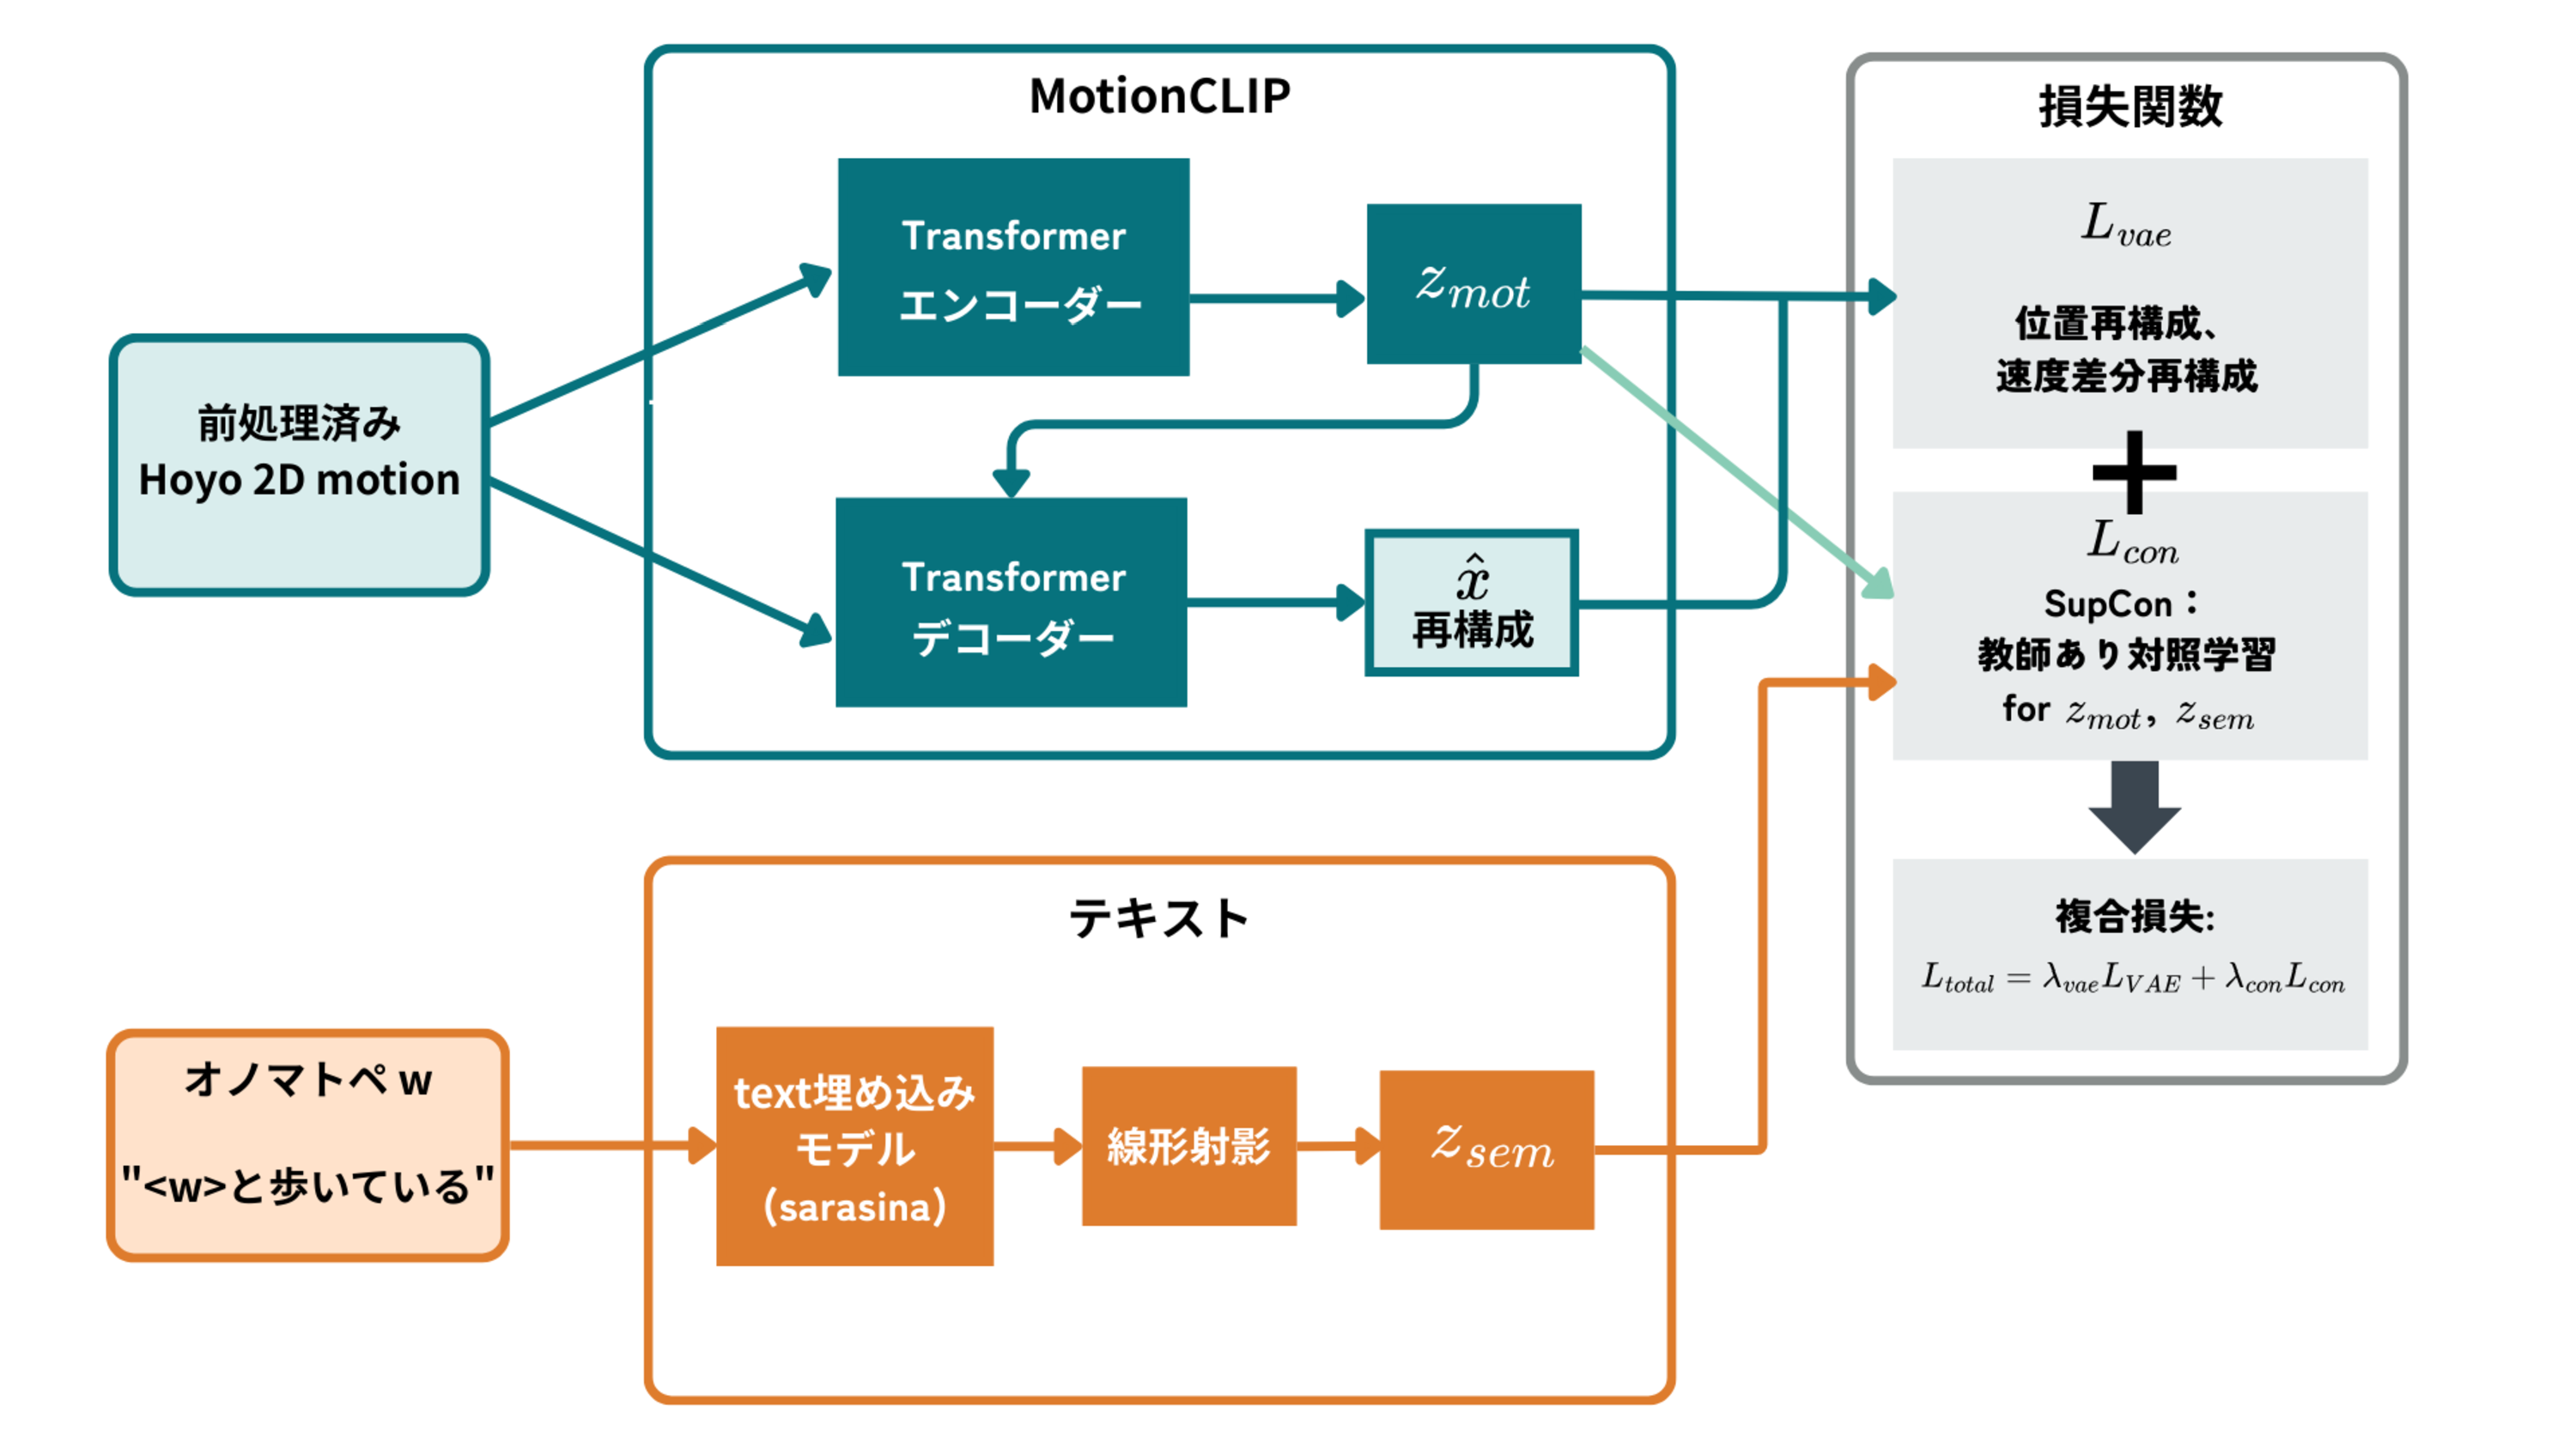
\includegraphics[width=\textwidth]{figs/3/Phase1.pdf}
  \caption{Phase 1 の全体フロー}
  \label{fig:phase1_contrastive_learning}
\end{figure}

\subsection{モデル構成}
\label{subsec:offline_model}

MotionCLIP \cite{MotionCLIP} の Transformer ベース VAE を 2D 歩容系列に合わせて再利用する．
MotionCLIP は本来 3D（$xyz$）の関節表現を前提とするが，
本研究では 3D 再構成を行わず，観測可能な 2D 座標（$xy$）に射影した系列を入力として扱う．
入力・出力は $(T^\ast, 14, 2)$ に合わせる．
ここで $T^\ast$ は前処理後の固定フレーム長を表し，
リサンプリング後にクロップ／パディングして揃える．
本研究では $T^\ast=100$ とする．
エンコーダ $f_{\mathrm{enc}}$ は
\begin{align}
  z_{\mathrm{mot}} = \mathrm{normalize}\left(f_{\mathrm{enc}}(\tilde{X})\right)
\end{align}
を出力し，デコーダ $f_{\mathrm{dec}}$ は系列を再構成する．
再構成損失の定義は後述する（式\ref{eq:proposed_vae_2d}）．

\paragraph{2D 表現への適用}\quad\\

各フレームの 2D 関節座標をベクトル化し，線形射影で埋め込み次元へ写像する．
時間方向には位置埋め込みを加え, Transformer により文脈化する．
MotionCLIP の 3D 関節回転やメッシュ頂点に基づく項はHOYO datasetが2D データのため用いず，
2D 系列の再構成（位置 + 速度差分）に合わせた損失で学習する．

\paragraph{テキスト埋め込み}\quad\\

オノマトペ $w$ はテンプレート文に埋め込み，意味ベクトルを得る．
\begin{center}
  \texttt{「<w>と歩いている。」}\\
  （ただし $w=\text{通常}$ のときは「普通に歩いている。」）
\end{center}
Sarashina \cite{sarashina} または SigLIP \cite{siglip} を用い，
\begin{align}
  u_{\mathrm{sem}} = e_{\mathrm{text}}(\mathrm{text}(w))
\end{align}
を計算する．


\paragraph{意味射影}\quad\\

テキスト埋め込みを MotionCLIP 潜在空間に合わせるため，線形射影
\begin{align}
  z_{\mathrm{sem}} = \mathrm{normalize}\left(W u_{\mathrm{sem}}\right),\quad W\in\mathbb{R}^{D\times D_{\mathrm{sem}}}
\end{align}
を導入する（バイアスなし）．温度パラメータは $\tau = \exp(-\alpha)$ とし，$\alpha$ を学習する．

\paragraph{再構成損失}\quad\\

本研究では 2D 関節座標の再構成と速度（差分）再構成からなる損失を
$\mathcal{L}_{\mathrm{VAE}}$ として用いる（2章 式\ref{eq:motionclip_recon} と同様）．
\begin{align}
  \mathcal{L}_{\mathrm{VAE}}
   & = \frac{1}{JT^\ast}\sum_{t=1}^{T^\ast}\sum_{j=1}^{J}\|x_{t,j} - \hat{x}_{t,j}\|^2 \notag \\
   & \quad + \frac{1}{J(T^\ast-1)}\sum_{t=1}^{T^\ast-1}\sum_{j=1}^{J}
  \|(x_{t+1,j}-x_{t,j})-(\hat{x}_{t+1,j}-\hat{x}_{t,j})\|^2
  \label{eq:proposed_vae_2d}
\end{align}

\paragraph{対照損失}\quad\\

対照損失には教師あり対照学習 SupCon \cite{supcon} を用いる．
バッチ内のモーション潜在 $z_{\mathrm{mot}}$ と同一ラベルの意味潜在 $z_{\mathrm{sem}}$ を正例として扱い，
異ラベルを負例とする教師あり対照学習を行う．
ここで，同一オノマトペで被験者が異なるサンプルも同じ正例群として扱うため，
個体固有の差よりも語彙に共通する歩容スタイル特徴を優先して表現する方向に学習が進む．
\begin{align}
  \mathcal{L}_{\mathrm{con}}
  =
  -\sum_i \frac{1}{|P(i)|}
  \sum_{p\in P(i)}
  \log
  \frac{\exp\!\left(\mathrm{sim}(z_i,z_p)/\tau\right)}
       {\sum_{a\in A(i)} \exp\!\left(\mathrm{sim}(z_i,z_a)/\tau\right)}
\end{align}
ここで，$P(i)$ はアンカー $i$ と同一ラベルの正例集合，
$A(i)$ はバッチ内の比較対象集合，$\mathrm{sim}(\cdot,\cdot)$ はコサイン類似度，$\tau$ は温度パラメータである．

最終損失は
\begin{align}
  \mathcal{L}_{\mathrm{total}}
  = \lambda_{\mathrm{vae}}\,\mathcal{L}_{\mathrm{VAE}} + \lambda_{\mathrm{con}}\,\mathcal{L}_{\mathrm{con}}
\end{align}
で与える．
なお \textbf{freeze 段階では $\lambda_{\mathrm{vae}}=0$} とし，対照損失のみで射影層を学習する．

\subsection{学習手順}
\label{subsec:offline_train}

学習は段階的に進める．
\begin{itemize}
  \item \textbf{freeze}：MotionCLIP の encoder/decoder を固定し，$W$ と温度 $\alpha$ のみ更新．
  \item \textbf{full}：encoder/decoder をともに fine-tune．
\end{itemize}
各段階の開始時に，前段の最良モデルをロードして初期値とする．

データはラベルごとに 8:2 で分割する．
学習には AdamW を用い，クラス不均衡を補正するために \textbf{WeightedRandomSampler} を用いてバッチを構成する．

評価には検索指標（R@K，MedR）および silhouette を用いる．

\section{強化学習によるスタイル制御（Phase 2）}
\label{sec:online_phase}

Phase 2 におけるリターゲット，スタイル報酬計算，および PPO による方策更新の関係を
図\ref{fig:phase2_style_reward_rl}に示す．

\begin{figure}[htbp]
  \centering
  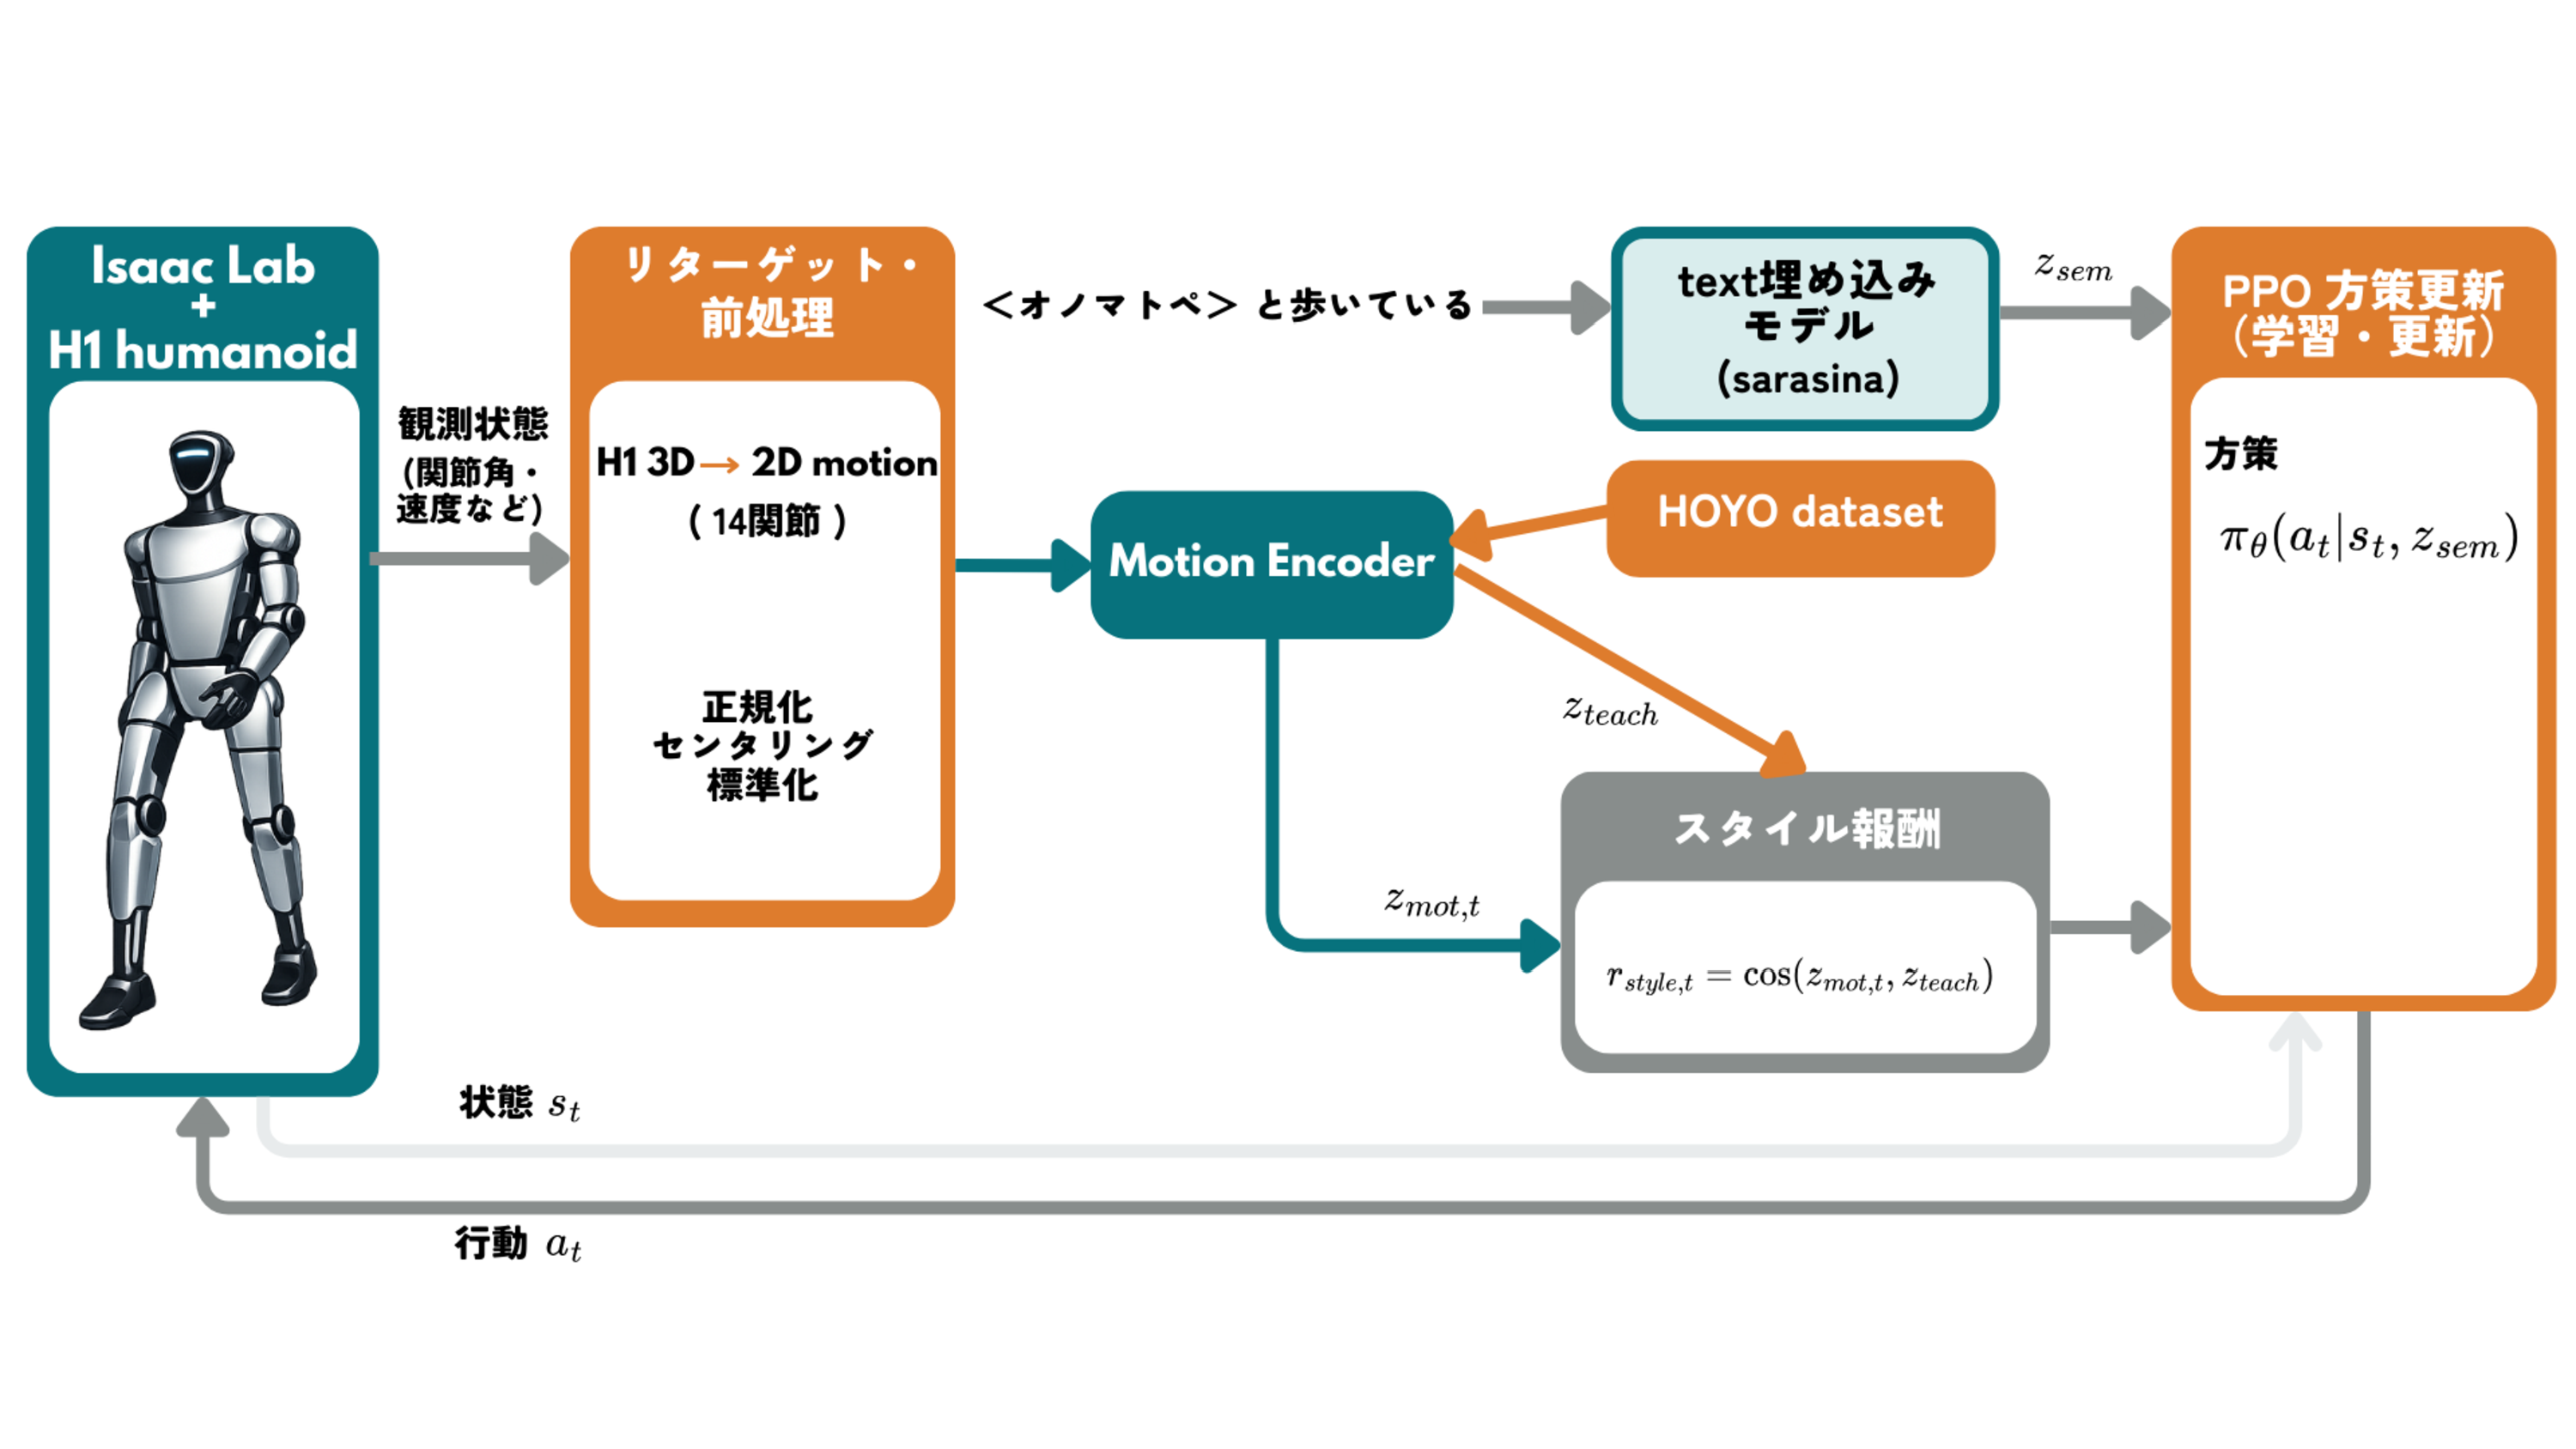
\includegraphics[width=\textwidth]{figs/3/Phase2.pdf}
  \caption{Phase 2 の全体フロー}
  \label{fig:phase2_style_reward_rl}
\end{figure}

\subsection{リターゲットと潜在推定}
\label{subsec:rl_retarget}

物理シミュレータ上のロボットの動作を，Phase 1 で学習した潜在空間へ写像するため，
オンラインでのリターゲットおよび MotionCLIP エンコーダによる潜在表現の推定を行う．

\paragraph{関節対応と座標変換}\quad\\

3 次元ヒューマノイドロボット（H1）の関節位置情報を，HOYO データセットで定義される 2 次元スケルトン形式へ変換する．
H1 の特定の関節位置を HOYO の対応する 14 関節にマッピングし，
ロボットの進行方向が正対するように座標軸の変換（$Y_{\mathrm{H1}} \to x_{\mathrm{HOYO}},\ -Z_{\mathrm{H1}} \to y_{\mathrm{HOYO}}$）を行う．
これにより，3 次元空間での歩行動作を，Phase 1 のエンコーダが解釈可能な 2 次元正面視点の系列として扱う．

\paragraph{正規化と入力系列の構成}\quad\\

変換された系列は，初期フレームの重心でセンタリングし，2 次元へ投影したのち，
身長正規化と平均・標準偏差による標準化に加えて，常に Yaw 補正を適用する．
Yaw 補正では，ベースのヨー角を打ち消す回転を各フレームに与え，進行方向を正面基準に整列させる．
これは，HOYO データセットがカメラ正面方向への歩行を主対象とし，横移動を含まない条件で構成されているためである．
シミュレータ側もこの条件に合わせて横方向成分の影響を抑え，前後方向の歩容差を主に比較できるようにする．
その上で，直近 $L$ フレームの関節系列を履歴バッファとして保持し，
バッファが揃った時点からエンコーダ $f_{\mathrm{enc}}$ に入力して
動作潜在 $z_{\mathrm{mot}, t}$ を逐次計算する．

\subsection{方策の条件付けと報酬設計}
\label{subsec:rl_reward}

本研究では，タスク達成（安定歩行・前進維持）とスタイル表現を両立させるため，
オノマトペ埋め込みベクトルによる方策の条件付けと，潜在空間上の類似度に基づく報酬設計を行う．

\paragraph{オノマトペ埋め込みベクトルと方策入力}\quad\\

エピソードごとにオノマトペ $w$ をサンプリングし，そのテキスト埋め込みから得られる意味潜在ベクトル $z_{\mathrm{sem}}$ をオノマトペ埋め込みベクトルとする（Phase 1 と同じ記号を用いる）．
方策ネットワークには，ロボットの観測状態 $s_t$（関節角度・速度等）に加え，
この $z_{\mathrm{sem}}$ を条件として入力する．
これにより，入力されたオノマトペに応じて異なる歩容を生成可能な方策を学習する．

\paragraph{報酬関数の構成}\quad\\

報酬関数 $r_t$ は，基本的な歩行タスクを評価する $r_{\mathrm{task}}$ と，
スタイルの整合性を評価する $r_{\mathrm{style}}$ の加重和で定義する．
\begin{align}
  r_t = r_{\mathrm{task}, t} + w_{\mathrm{style}}(n)\, r_{\mathrm{style}, t}
\end{align}
ここで $w_{\mathrm{style}}(n)$ は学習初期の転倒を避けるための重みスケジュールであり，
学習ステップ $n$ に対して 0 から所定の上限へ線形に増加させる（例：$w_{\mathrm{style}}(n)=\min\{w_{\max},\,n/T_{\mathrm{ramp}}\cdot w_{\max}\}$）．

\paragraph{タスク報酬 ($r_{\mathrm{task}}$)}\quad\\

転倒を避けつつ前進歩行を維持し，スタイル報酬のみでその場足踏みに収束することを防ぐための報酬項である．
本研究では NaVILAのlow-levl policy\cite{NaVILA_paper}）に基づき，タスク報酬を
\begin{align}
  r_{\mathrm{task},t} = \sum_{k \in \mathcal{K}_{\mathrm{task}}} w_k\,\phi_k(s_t, a_t)
  \label{eq:task_reward_sum}
\end{align}
の重み付き和で与える（係数 $w_k$ は表\ref{tab:reward_main}および表\ref{tab:reward_reg}に示す）．

以下に，本研究で用いた主要な項 $\phi_k$ を実装に沿って定義する．

\paragraph{Linear Velocity Tracking (XY) / Heading Tracking (World Yaw)}\quad\\

ロボットのベース速度が与えた速度条件から極端に外れない度合いを指数カーネルで評価する．
まず，平面並進の指令速度を $c^{\mathrm{lin}}_t = [v^{\mathrm{cmd}}_{x,t}, v^{\mathrm{cmd}}_{y,t}]$ とし，
ベース線速度 $v_t$ をヨー角のみを用いたロボット座標系（Yaw frame）へ変換したものを $v^{\mathrm{yaw}}_t$ とする．
このとき線速度追従報酬を
\begin{align}
  \phi_{\mathrm{lin},t} = \exp\!\left(-\frac{\|c^{\mathrm{lin}}_t - [v^{\mathrm{yaw}}_{x,t}, v^{\mathrm{yaw}}_{y,t}]\|^2}{\sigma_{\mathrm{lin}}^2}\right)
  \label{eq:task_track_lin}
\end{align}
とする．
本項の役割は厳密な速度一致の達成ではなく，足踏み解を避けながら語彙間の速度差が発現できる前進条件を与えることにある．

次に，ワールド座標系での目標方位（heading）$\psi^{\mathrm{target}}$ に対する追従項を
\begin{align}
  \phi_{\mathrm{head},t}
  =
  \exp\!\left(
  -\frac{\operatorname{wrapTo\pi}(\psi_t-\psi^{\mathrm{target}})^2}{\sigma_{\mathrm{head}}^2}
  \right)
  \label{eq:task_track_heading}
\end{align}
で定義する（本研究の比較設定では $\psi^{\mathrm{target}}=0$）．
ここで $\psi_t$ はベースのワールド座標系ヨー角，
$\sigma_{\mathrm{lin}},\sigma_{\mathrm{head}}$ は各追従項のカーネル幅である．
なお，NaVILA の原論文では $z$ 軸角速度への追従（Angular velocity tracking）が用いられているが，
本研究では直進歩行における方位保持を重視し，目標ヨー角への追従（Heading Tracking）に置き換えている．

\paragraph{Flat Orientation}\quad\\

体幹が傾きすぎないよう，重力の射影ベクトル $g^{\mathrm{proj}}_t$ の水平成分を二乗ノルムで罰する．
\begin{align}
  \phi_{\mathrm{ori},t} = \|[g^{\mathrm{proj}}_{x,t}, g^{\mathrm{proj}}_{y,t}]\|^2
  \label{eq:task_flat_ori}
\end{align}

\paragraph{Angular Velocity Penalty (XY)}\quad\\

不要なロール・ピッチ方向の回転を抑えるため，ベース角速度の水平成分を二乗ノルムで罰する．
\begin{align}
  \phi_{\mathrm{ang},t} = \|[\omega_{x,t}, \omega_{y,t}]\|^2
  \label{eq:task_ang_vel_xy}
\end{align}
なお，元論文では鉛直方向の線速度ペナルティ（$v_{z,t}^2$）も用いられるが，本研究の二足歩行設定では当該項は無効化している．

\paragraph{Action Rate Penalty / Joint Accelerations / \\ Joint Torques (Energy Proxy)}\quad\\

過度なトルクや関節加速度，急激な出力変化を抑制するため，以下のペナルティ項を用いる．
\begin{align}
  \phi_{\tau,t} &= \sum_{i\in\mathcal{J}} \tau_{t,i}^2, \\
  \phi_{\ddot{q},t} &= \sum_{i\in\mathcal{J}} \ddot{q}_{t,i}^2, \\
  \phi_{\Delta a,t} &= \|a_t - a_{t-1}\|^2
  \label{eq:task_regs}
\end{align}
ここで $\mathcal{J}$ は対象とする関節集合であり，$\tau_{t,i}$ は関節 $i$ に加えたトルク，$\ddot{q}_{t,i}$ は関節加速度，
$a_t$ は方策ネットワークの出力アクションである．

\paragraph{Feet Air Time}\quad\\

すり足を防ぎ，左右の脚が交互に離地する歩容を促すための報酬項である．
各足 $f$ について，接触センサに基づく\textbf{モード時間} $t_{t,f}^{\mathrm{mode}}$ を定義する．
これは，接地中の足には接触継続時間を，遊脚には離地継続時間をそれぞれ割り当てたものである．
\textbf{片足のみ接地}（single-stance）の場合に限り，
左右のモード時間の最小値を上限 $t_{\max}$ でクリップして報酬とする：
\begin{align}
  \phi_{\mathrm{air},t} = \min\{t_{\max},\ \min_{f\in\{L,R\}} \;t_{t,f}^{\mathrm{mode}}\}\ \cdot\ \mathbf{1}[\|[v^{\mathrm{cmd}}_{x,t}, v^{\mathrm{cmd}}_{y,t}]\|>\epsilon],
  \label{eq:task_air_time}
\end{align}
ここで $\mathbf{1}[\cdot]$ は指示関数であり，
$\epsilon$ は速度指令がほぼゼロ（静止状態）のときに本報酬を無効化するための閾値である．

\paragraph{Feet Slipping Penalty}\quad\\

足裏が接地しているにもかかわらず水平に滑ることを抑制するため，
接地判定 $\mathbf{1}[\mathrm{contact}]$ と足部の水平速度 $\|\dot{p}_{t,f,xy}\|$ の積をペナルティとする：
\begin{align}
  \phi_{\mathrm{slide},t} = \sum_{f\in\{L,R\}} \|\dot{p}_{t,f,xy}\|\;\mathbf{1}[\mathrm{contact}_f].
  \label{eq:task_feet_slide}
\end{align}

\paragraph{DOF Position Limits Penalty / Joint Deviation (Hip/Arms/Torso)}\quad\\

足首関節など一部の関節について，ソフト可動域 $[\underline{q}^{\mathrm{soft}}_i, \overline{q}^{\mathrm{soft}}_i]$ を超えた分を罰する：
\begin{align}
  \phi_{\mathrm{lim},t} = \sum_{i\in\mathcal{J}_{\mathrm{ankle}}}
  \max\{0,\ q_{t,i}-\overline{q}^{\mathrm{soft}}_i\} + \max\{0,\ \underline{q}^{\mathrm{soft}}_i-q_{t,i}\}.
  \label{eq:task_joint_limits}
\end{align}
また，歩行に本質的でない関節（例：腕・体幹・股関節の一部）がデフォルト姿勢から逸脱しすぎないよう，L1 で抑制する：
\begin{align}
  \phi_{\mathrm{dev},t} = \sum_{i\in\mathcal{J}_{\mathrm{aux}}} \left|q_{t,i} - q^{\mathrm{default}}_i\right|.
  \label{eq:task_joint_dev}
\end{align}

\paragraph{Termination Penalty / Feet Stumble Penalty}\quad\\

エピソード終了（転倒等）にはペナルティを与える．また，足部の水平接触力が鉛直接触力に比べて過度に大きい場合を「つまずき」とみなし，
\begin{align}
  \phi_{\mathrm{term},t} &= \mathbf{1}[\mathrm{terminated}], \\
  \phi_{\mathrm{stumble},t} &= \mathbf{1}\!\left[\exists f\in\{L,R\}:\ \|F_{t,f,xy}\| > 5\,|F_{t,f,z}|\right]
  \label{eq:task_term_stumble}
\end{align}
を用いる．

\paragraph{Style Tracking (Teach)}\quad\\

生成された動作が目標スタイルに対応しているかを評価する．
直近 $L$ フレームから推定した動作潜在 $z_{\mathrm{mot},t}$ と，
目標オノマトペ $w$ に対応する教師潜在 $z_{\mathrm{teach}}(w)$ のコサイン類似度を用いる．
ここで $z_{\mathrm{teach}}(w)$ は，HOYO の教師 motion（ラベル $w$）を Phase 1 のエンコーダに通して得た潜在表現として事前に計算しておく．
なお，$z_{\mathrm{mot},t}$ および $z_{\mathrm{teach}}$ は L2 正規化済みであるため，内積がコサイン類似度と一致する．
\begin{equation}
  r_{\mathrm{style}, t}^{\mathrm{raw}}
  = \beta_{\mathrm{teach}}\cos(\tilde{z}_{\mathrm{mot}, t}, \tilde{z}_{\mathrm{teach}}(w))
  \label{eq:rl_style_raw}
\end{equation}

スタイル報酬は学習初期の過度な拘束による転倒を防ぐため，学習ステップ $n$ に応じて徐々に有効化する．

\begin{align}
  w_{\mathrm{style}}(n)=\min\!\left\{w_{\max},\ \frac{n}{T_{\mathrm{ramp}}}w_{\max}\right\}
  \label{eq:rl_style_ramp}
\end{align}

よって最終的な 1 ステップ報酬は

\begin{align}
  r_t = r_{\mathrm{task},t} + w_{\mathrm{style}}(n)\, r_{\mathrm{style}, t}^{\mathrm{raw}}
  \label{eq:rl_total_reward}
\end{align}

で与える．

\subsection{PPO による方策更新}
\label{subsec:rl_ppo_update}

方策更新には PPO \cite{PPO} を用いる．
現在方策と収集時方策の尤度比を
\begin{align}
  \rho_t(\theta)=\frac{\pi_\theta(a_t|s_t)}{\pi_{\theta_{\mathrm{old}}}(a_t|s_t)}
\end{align}
とすると，クリップ付き目的は
\begin{align}
  \mathcal{L}_{\mathrm{clip}}(\theta)
  =
  \mathbb{E}_t\!\left[
  \min\!\left(
  \rho_t(\theta)\hat{A}_t,\ 
  \mathrm{clip}(\rho_t(\theta),1-\epsilon,1+\epsilon)\hat{A}_t
  \right)\right]
  \label{eq:rl_ppo_clip}
\end{align}
となる．
実装では価値関数損失とエントロピー正則化を加えた目的を最大化する（2章 \ref{subsec:PPO} 節）．

\subsection{Phase 2 の学習手順}
\label{subsec:rl_train_flow}

Phase 2 の学習は以下の手順で行う．
\begin{enumerate}
  \item Phase 1 で学習したエンコーダ $f_{\mathrm{enc}}$ を固定し，オノマトペ埋め込みベクトルを準備する．
  \item エピソード開始時にオノマトペ $w$ をサンプリングし，対応するオノマトペ埋め込みベクトル（$z_{\mathrm{sem}}(w)$）を方策入力へ付与する．
  \item 各ステップでロボット状態を観測し，方策 $\pi_\theta(a_t|s_t, z_{\mathrm{sem}})$ から行動を生成する．
  \item リターゲット後の 2D 関節系列から $z_{\mathrm{mot},t}$ を推定し，式\ref{eq:rl_style_raw}--\ref{eq:rl_total_reward} により報酬を計算する．
  \item 一定長のロールアウトを収集後，GAE でadvantageを推定し，式\ref{eq:rl_ppo_clip} に基づいて方策・価値関数を更新する．
\end{enumerate}

この更新を反復することで，前進維持と転倒回避を満たしつつ，オノマトペ条件に応じた歩容の生成を目指す．
